\documentclass[11pt,oneside,a4paper]{book}

\usepackage[a4paper,margin=25mm,top=30mm,bottom=30mm]{geometry}
\usepackage{graphicx}
\usepackage{inconsolata}
\usepackage[T1]{fontenc}
\usepackage{hyperref}
\hypersetup{colorlinks=true,allcolors=blue}
\usepackage{fancyhdr}
\usepackage{color, xcolor}
\usepackage{titlesec}
\usepackage{float}
\usepackage{listings}
\usepackage{booktabs, longtable}
\usepackage{enumitem}

\setlist[itemize, 1]{label=$\color{DarkGreen}\bullet$}
\setlist[itemize, 2]{label=\tiny\textbullet}

\definecolor{NavyBlue}{RGB}{18, 28, 97}
\definecolor{CyberTeal}{RGB}{0, 130, 130}
\definecolor{SecurityGreen}{RGB}{67, 160, 71}
\definecolor{AlertOrange}{RGB}{251, 140, 0}
\definecolor{DangerRed}{RGB}{229, 57, 53}
\definecolor{CodeBackground}{RGB}{245, 245, 245}
\definecolor{DarkGrayText}{RGB}{60, 60, 60}

\colorlet{ChapterColor}{NavyBlue}
\colorlet{SectionColor}{NavyBlue}
\colorlet{SubsectionColor}{CyberTeal}
\colorlet{CodeColor}{DarkGrayText}
\colorlet{KeywordColor}{NavyBlue}
\colorlet{CommentColor}{SecurityGreen}
\colorlet{StringColor}{DangerRed}

\pagestyle{fancy}
\fancyhf{}
\fancyfoot[C]{\textcolor{DarkGrayText}{\footnotesize Confidential — Page \thepage}}
\renewcommand{\headrulewidth}{0.8pt}
\fancyhead[L]{\rightmark}

\titleformat{\chapter}[display]
  {\normalfont\bfseries\Huge\color{ChapterColor}\raggedright}
  {\MakeUppercase{\chaptertitlename}\ \thechapter}{20pt}{\Huge}
\titlespacing*{\chapter}{0pt}{-30pt}{40pt}

\titleformat{\section}
  {\normalfont\Large\bfseries\color{SectionColor}}
  {\thesection}{1em}{}
\titlespacing*{\section}{0pt}{15pt}{10pt}

\titleformat{\subsection}
  {\normalfont\large\bfseries\color{SubsectionColor}}
  {\thesubsection}{1em}{}
\titlespacing*{\subsection}{0pt}{12pt}{8pt}

\lstset{
  backgroundcolor=\color{CodeBackground},
  basicstyle=\footnotesize\ttfamily\color{CodeColor},
  keywordstyle=\bfseries\color{KeywordColor},
  commentstyle=\color{CommentColor}\textit,
  stringstyle=\color{StringColor},
  frame=tb,
  framerule=0.5pt,
  rulesepcolor=\color{LightGray},
  breaklines=true,
  postbreak=\mbox{\color{DangerRed}\space\small$\hookleftarrow$},
  numberstyle=\tiny\color{gray},
  numbers=left,
  stepnumber=1,
  numbersep=5pt,
  showspaces=false,
  showstringspaces=false,
  showtabs=false,
  tabsize=2,
  captionpos=b,
  framextopmargin=5pt, framexbottommargin=5pt
}

\newcommand{\extensionname}{Password Security Checker}
\newcommand{\esia}{\textit{ENSIA}}

\begin{document}
\begin{titlepage}
  \centering
  \vspace*{3cm}
  
\includegraphics[width=0.4\textwidth]{logo.png}\\[1.5em]
  {\Huge\bfseries\color{ChapterColor}\extensionname\ Final Report}\\[3em]

  {\bfseries Team Members:}\\[0.5em]
  Imene Fatma DJELILI\\[0.05em]
  Hadil HATTABI\\[0.05em]
  Firdaws BASSAID\\[0.05em]
  Hachem Safi Eddine SEKHSOUKH\\[0.05em]
  Youcef GUERGOUR\\[0.05em]
  Rafik MESSAOUD NACER\\[4em]

  \vfill

  {\Large Submitted to \esia}\\[0.5em]
  {\normalsize Project ID: [S004]}\\[1em]
  {\normalsize Version: 1.0}\\[0.5em]
  {\normalsize Date: \today}
\end{titlepage}

\frontmatter
\tableofcontents
\newpage

\chapter*{Confidentiality Statement}
\addcontentsline{toc}{chapter}{Confidentiality Statement}
This document and all the content herein are confidential and intended solely for academic evaluation within the École Nationale Supérieure d'Intelligence Artificielle (\esia).

The \extensionname\ project presented in this document contains technical and innovative information developed as part of an academic exercise.

By accessing this document, the reader agrees to respect the confidentiality of the information provided and acknowledges that it is solely for academic assessment under the supervision of \esia faculty members.

\section*{Disclaimer}
\addcontentsline{toc}{section}{Disclaimer}
The implementation and technical details presented in this report pertain specifically to the state of the \extensionname\ Extension as developed and finalized at the conclusion of Semester 2 of the 2024/2025 academic year.

This document reflects the knowledge, tools, and methodologies available to the project team during that period. As such, any future enhancements, modifications, or deviations from the described functionalities are not covered within the scope of this report. The information contained herein is accurate to the best of the team's understanding at the time of submission and is intended solely for academic evaluation purposes.

\chapter*{Contact Information}
\addcontentsline{toc}{chapter}{Contact Information}
\begin{longtable}{|p{4cm}|p{4cm}|p{7cm}|}
\hline
\textbf{First Name} & \textbf{Last Name} & \textbf{Email} \\
\hline
Imene Fatma & DJELILI & \href{mailto:fatma.imene.djelili@ensia.edu.dz}{fatma.imene.djelili@ensia.edu.dz} \\
Hadil & HATTABI & \href{mailto:hadil.hattabi@ensia.edu.dz}{hadil.hattabi@ensia.edu.dz} \\
Firdaws & BASSAID & \href{mailto:firdaws.bassaid@ensia.edu.dz}{firdaws.bassaid@ensia.edu.dz} \\
Hachem Safi Eddine & SEKHSOUKH & \href{mailto:hachem.safi.eddine.sekhsoukh@ensia.edu.dz}{hachem.safi.eddine.sekhsoukh@ensia.edu.dz} \\
Youcef & GUERGOUR & \href{mailto:youcef.guergour@ensia.edu.dz}{youcef.guergour@ensia.edu.dz} \\
Rafik & MESSAOUD NACER & \href{mailto:rafik.messaoud.nacer@ensia.edu.dz}{rafik.messaoud.macer@ensia.edu.dz} \\
\hline
\end{longtable}

\mainmatter

\chapter{Introduction}
In the ever-evolving digital landscape, the security of online accounts hinges critically on the strength and uniqueness of passwords. Unfortunately, common user practices, such as password reuse, selection of easily guessable combinations, and unawareness of credentials exposed in data breaches, pose significant vulnerabilities. These behaviors expose individuals and organizations alike to prevalent cyber threats, including credential stuffing, brute-force attacks, and phishing campaigns leveraging leaked data.

Addressing this critical security gap, the \extensionname\ is designed as an intelligent, cross-browser compatible web extension aimed at empowering users through education and real-time feedback on password security during interactions with online forms. The extension seamlessly integrates into the browsing experience, automatically detecting password input fields and providing immediate insights into a password's robustness and associated risks.

Utilizing a multi-faceted approach, the extension evaluates passwords against key security indicators:
\begin{itemize}
    \item Real-time strength assessment considering length, character composition, and entropy.
    \item Detection of usage patterns susceptible to simulated common cracking techniques.
    \item Identification of previous usage across different online services.
    \item Cross-referencing against databases of credentials exposed in public data breaches via a secure, privacy-preserving method.
    \item Enforcement of minimum security criteria before form submission.
    \item Integration of \esia branding to foster trust and recognition.
\end{itemize}
By providing clear visual indicators, detailed explanations in its popup interface, and proactive notifications for serious vulnerabilities, \extensionname\ serves as a vital tool for improving user password hygiene and strengthening overall online security posture. This report details the objectives, technical implementation, core features, and cross-browser compatibility of the developed extension.

\chapter{Objectives}
The core objective of the \extensionname\ project is to serve as a proactive browser-based security assistant, significantly improving user password security hygiene. This overarching goal is broken down into the following key objectives:

\section{Real-time Password Analysis and Enforcement}
To automatically identify password fields on webpages and provide users with instant, dynamic feedback as they type. This feedback assesses the password based on critical security metrics like length, character variety, and randomness (entropy). A primary goal is also to introduce a layer of enforcement, preventing the submission of passwords that fail to meet defined security thresholds, thereby encouraging the creation and use of stronger credentials.

\section{Comprehensive Vulnerability Assessment}
To go beyond basic strength scoring by implementing checks against known weaknesses. This includes detecting patterns vulnerable to common cracking methods (simulated locally), identifying instances where a password has been reused across multiple sites (tracked locally and via known breaches), and leveraging external services (like Have I Been Pwned) to alert users if their password has appeared in public data breaches.

\section{Intuitive User Guidance and Notification}
To present complex security information in an accessible, user-friendly manner through a clear popup interface and integrated visual cues directly on the webpage. Critical alerts, such as the detection of an easily "crackable" password or a known breach compromise, will be delivered through prominent browser notifications, ensuring the user is promptly informed of significant risks and guided towards safer password practices.

\section{Broad Browser Accessibility}
To develop the extension with a focus on cross-browser compatibility, ensuring reliable performance and consistent functionality across major platforms, including Chrome, Firefox, Edge, and Safari. This objective involves careful architectural design and implementation techniques to abstract browser-specific APIs and behaviors.

\section{Reinforcement of Security Best Practices}
To integrate guidance and educational tips directly into the user experience, helping users understand *why* certain passwords are weak and *how* to create stronger, more secure ones. This includes actionable advice like suggesting combinations of characters, promoting password manager usage, and emphasizing the importance of unique passwords for every service.

By achieving these objectives, \extensionname\ aims to transform passive password usage into an informed and actively secured process for every user.

\chapter{Key Features}
The \extensionname\ provides a suite of features designed to offer users comprehensive, real-time feedback and security enforcement for their passwords. These features are seamlessly integrated into the browsing experience.

\section{Real-time Strength Assessment and Enforcement}
This feature provides instant feedback on password quality and prevents the use of overtly weak credentials on web forms.

\subsection{User Perspective}
As a user types into a password field, a small icon appears nearby, changing color (e.g., red for weak, green for strong) based on the password's quality. Hovering over the icon displays a detailed explanation in a tooltip, highlighting specific issues and offering improvement suggestions. If attempting to submit a form with a password deemed too weak according to predefined rules, the extension blocks the submission and presents an error message.

\subsection{Technical Implementation}
\subsubsection{Password Field Detection and Monitoring}
The \texttt{content.js} script is injected into every webpage and uses DOM querying\\
 (\texttt{document.querySelectorAll('input[type="password"]')}) to find password fields.\\ A \texttt{MutationObserver} is also employed to detect fields added dynamically by JavaScript after the initial page load.
\begin{lstlisting}[language=JavaScript, caption=Content Script MutationObserver for Dynamic Fields]
const observer = new MutationObserver(mutations => {
    mutations.forEach(mutation => {
        if (mutation.addedNodes && mutation.addedNodes.length > 0) {
            mutation.addedNodes.forEach(node => {
                if (node.nodeType === 1 && (node.matches('input[type="password"]') || node.querySelector('input[type="password"]'))) {
                    detectPasswordFields();
                }
            });
        }
    });
});
observer.observe(document.body, { childList: true, subtree: true });
\end{lstlisting}
An `input` event listener is attached to each detected password field. When the user types, the password value is sent to the \texttt{background.js} script for detailed validation via\\ `chrome.runtime.sendMessage`. A debounce function is used to limit validation requests and improve performance, preventing checks on every single keystroke.

\subsubsection{Background Validation Logic}
The \texttt{background.js} script handles the primary validation through the \texttt{safeValidatePassword} function. This function assesses the password against several criteria:
\begin{itemize}
    \item \textbf{Length:} Checks if the password meets the minimum required length\\ (\texttt{PASSWORD\_REQUIREMENTS.minLength}).
    \item \textbf{Complexity:} Verifies the presence of uppercase letters, lowercase letters, numbers, and special characters based on \texttt{PASSWORD\_REQUIREMENTS} flags.
    \item \textbf{Entropy:} Calculates the Shannon entropy of the password using \texttt{calculateEntropy}, which measures the theoretical randomness based on character set size and length.
    \begin{lstlisting}[language=JavaScript, caption=Entropy Calculation]
function calculateEntropy(password) {
    let charset = 0;
    if (/[a-z]/.test(password)) charset += 26;
    if (/[A-Z]/.test(password)) charset += 26;
    if (/[0-9]/.test(password)) charset += 10;
    if (/[^a-zA-Z0-9]/.test(password)) charset += 32;
    if (charset === 0) return 0;
    return Math.log2(Math.pow(charset, password.length));
}
    \end{lstlisting}
    These criteria align with widely accepted guidelines for password security, such as principles found in NIST or OWASP recommendations, aiming to create passwords that are resistant to brute force and guessing.
\end{itemize}
The background script returns a detailed response object including a boolean \texttt{isValid}, the calculated \texttt{entropy}, and a consolidated \texttt{feedback} string listing all identified issues.

\subsubsection{UI Update and Enforcement}
The \texttt{content.js} script receives the validation response and updates the password field's appearance using \texttt{updatePasswordFieldStatus}. This involves adding visual indicators, applying CSS styles (e.g., border color), adjusting padding for the icon, and positioning the interactive tooltip showing the feedback message. The `passwordValidationStates` Map in \texttt{content.js} stores the validity status for each password field.

On forms containing password fields, the \texttt{content.js} adds a submit event listener. This listener prevents the default form submission and first triggers validation for all populated password fields on the form. After all validations return from the background script, it checks if every non-empty password field's state in \texttt{passwordValidationStates} is \texttt{true}. If any password is invalid, it blocks the submission, displays an error message at the top of the form, and prompts the user to fix the highlighted fields.
\begin{lstlisting}[language=JavaScript, caption=Content Script Form Submit Listener]
form.addEventListener('submit', async (e) => {
    e.preventDefault();
    const fields = form.querySelectorAll('input[type="password"]');
    const validationPromises = [];
    fields.forEach(field => {
        if (field.value) {
            validationPromises.push(validatePasswordWithExtension(field.value, field));
        }
    });
    await Promise.all(validationPromises);

    const allValid = Array.from(fields)
        .filter(field => field.value)
        .every(field => passwordValidationStates.get(field) === true);

    if (allValid) {
        form.submit();
    } else {
        displayFormErrorMessage(form, 'Please fix invalid passwords.');
    }
});
\end{lstlisting}

\section{Password Reuse Detection}
Preventing password reuse across multiple services is paramount to mitigating the impact of data breaches. This feature helps users avoid this dangerous practice.

\subsection{User Perspective}
When a password is entered and validated, the feedback provided in the tooltip and popup may include a warning if the password has been used on other websites the user has logged into while the extension is active, or if it has appeared in known global data breaches. The message clearly lists where else the password is known to be used (locally tracked) or how many times it appeared in breaches (from the external check).

\subsection{Technical Implementation}
\subsubsection{Local Reuse Check}
The \texttt{background.js} script's \texttt{checkPasswordReuse} function performs two checks. First, it queries the extension's local storage for previously saved password hashes and their associated domains (\texttt{chrome.storage.local.get(['passwordHistory'])}). Passwords are not stored in plain text but as cryptographic hashes (SHA-256 via \texttt{hashPassword}), ensuring privacy. The history tracks which domains a specific password hash (representing a unique password) has been associated with. If the current password's hash matches one in storage that is linked to *other* domains, a reuse warning is generated. The function \texttt{storePasswordUsage} updates this history upon successful validation of a new password for a given domain.

\subsubsection{Global Breach Check}
The second part of the reuse check involves querying the Have I Been Pwned (HIBP) API using a privacy-preserving k-anonymity technique (\texttt{checkHaveIBeenPwned}).
\begin{itemize}
    \item The password is first hashed using SHA-1 (\texttt{sha1}).
    \item Only the first 5 characters of the hash are sent to the HIBP API endpoint \\(\texttt{https://api.pwnedpasswords.com/range/{prefix}}).
    \item The API responds with a list of all hash suffixes that share that prefix, along with their breach counts.
    \item The extension then searches this list *locally* for the full hash's suffix.
\end{itemize}
This method ensures the HIBP service never receives the full password or its complete hash, preserving user privacy. If the suffix is found, the returned count indicates the number of times that password (hash) has appeared in public data breaches, and a corresponding warning is added to the validation issues.

\section{Password Cracking Simulation and Notification}
This feature simulates common offline password attacks locally to assess how quickly a password *could* theoretically be guessed and alerts the user to serious vulnerabilities.

\subsection{User Perspective}
If the extension's analysis determines that a password is vulnerable to common cracking methods (e.g., dictionary attacks, pattern matching, or very fast brute force for short passwords), the feedback will include an estimated time an attacker might take to crack it (e.g., "seconds", "minutes"). For passwords susceptible to rapid cracking or found via breached data, a prominent browser notification will appear, even if the user didn't click the popup. The notification urges the user to change the password immediately and is triggered periodically if the vulnerable password isn't changed.

\subsection{Technical Implementation}
The \texttt{PasswordCracker} class, initialized in \texttt{background.js}, contains methods to simulate common attacks:
\begin{itemize}
    \item \textbf{Common Patterns:} Checks against regular expressions representing frequently used password structures (\texttt{testPatterns}).
    \item \textbf{Substitution Attacks:} Simulates reversing common character substitutions (like '@' for 'a' or '3' for 'e') and checks if the resulting password is a common word or phrase (\texttt{testSubstitutions} leveraging \texttt{data/common\_passwords.csv}).
    \item \textbf{Keyboard Patterns:} Detects sequences like "qwerty" or "12345" (\texttt{testKeyboardPatterns}).
    \item \textbf{Date Patterns:} Looks for easily guessable date formats within the password\\ (\texttt{testDatePatterns}).
    \item \textbf{Time Estimation:} Calculates a theoretical cracking time based on the password's complexity and length, assuming modern cracking speeds (\texttt{estimateCrackingTime}). This is an estimate against offline brute force, not real-world online attacks.
\end{itemize}
When \texttt{safeValidatePassword} runs, it calls \texttt{passwordCracker.simulateCrack}. If the simulation returns \texttt{crackable: true}, indicating one of the simulation methods was successful or the password was deemed too short, this result is included in the feedback.

Furthermore, if a password is found to be crackable *or* if the HIBP check returns a breach count $> 0$, the \texttt{background.js} script triggers a standard browser notification using \texttt{browserAPI.notifications.create}. This ensures a user sees critical alerts even if they miss the on-page indicator or popup.

Passwords flagged as "crackable" are also stored locally (hashed) with a timestamp in the extension's storage (`crackedPasswords`). A periodic alarm (`chrome.alarms` for V3, `setInterval` for V2) triggers the \texttt{checkStoredCrackedPasswords} function in \texttt{background.js} daily. This function checks the `crackedPasswords` storage and issues a recurring notification every 7 days for any password that was previously flagged but hasn't been encountered as `isValid` since then, reminding the user to change it.

\section{ENSIA Branding Integration}
To align the extension with its origin and purpose within the \esia context, branding elements are incorporated into the user interface.

\subsection{User Perspective}
Users will see the distinct \esia logo integrated within the popup interface and the inline notification that appears on webpages, providing a recognizable visual cue associated with the institution.

\subsection{Technical Implementation}
The \esia logo (\texttt{icons/EnsiaLogo.png}) is included as an asset within the extension's project files. To display this image in HTML (e.g., \texttt{popup.html}) or dynamically add it via the content script (e.g., in the notification), the extension uses\\ \texttt{chrome.runtime.getURL('icons/EnsiaLogo.png')}. This function safely retrieves the path to the local extension resource.
\begin{lstlisting}[language=html, caption=ENSIA Logo in popup.html]
<div class="logo-container">
    <img src="icons/EnsiaLogo.png" alt="ENSIA Logo" class="ensia-logo">
</div>
\end{lstlisting}
The logo file must be listed in the \texttt{web\_accessible\_resources} section of the \texttt{manifest.json} for the content script to be able to load it into a webpage. CSS styling is applied (in \texttt{popup.css} and inline in \texttt{content.js}) to position and size the logo appropriately within the UI elements. The color palette used throughout the UI (blues, greens, reds for feedback) complements the branding and common cybersecurity visual language.

\chapter{Architecture and Implementation Details}
The \extensionname\ employs a standard browser extension architecture involving background and content scripts, managed via browser manifests and enabled for cross-browser compatibility through polyfilling.

\section{Cross-Browser Compatibility}
Achieving functionality across multiple browser engines requires addressing variations in their extension APIs and manifest versions.

\subsection{Implementation Strategy}
\subsubsection{Browser Polyfill}
The core strategy for handling API differences between Chrome (Manifest V3, primarily using `chrome.`) and Firefox/Safari (Manifest V2, primarily using `browser.` or `safari.`) is the inclusion of `browser-polyfill.js`. This script detects the available browser environment (\texttt{chrome}, \texttt{browser}, or \texttt{safari}) and creates a unified \texttt{browserAPI} object that provides a consistent interface for common operations like storage, messaging, tabs, and notifications, routing calls to the appropriate native API.
\begin{lstlisting}[language=JavaScript, caption=browser-polyfill.js Snippet]
const browserAPI = {
    api: null,
    browserType: null,
    init() { },
    async sendMessage(message) { },
    storage: { },
    notifications: { },
    tabs: { },
    extension: { }
};
browserAPI.init();
\end{lstlisting}
The polyfill is included in scripts where it's necessary to smooth out V2 API differences.

\subsubsection{Browser-Specific Manifests}
Separate manifest files (`manifest.json` for Chrome/Edge V3, `manifest.firefox.json` for Firefox V2, `manifest.safari.json` for Safari V2) are maintained. These files define browser-specific configurations such as:
\begin{itemize}
    \item \texttt{manifest\_version}.
    \item Background script definition.
    \item Browser action entry points.
    \item Permission syntax.
    \item Web accessible resources definition syntax.
    \item Content security policy (CSP) format.
\end{itemize}

\subsubsection{Build Process}
A Node.js build script (`build.js`) automates the process of packaging the extension for each target browser. It reads configuration for each browser (defined in the script), copies common source files into a browser-specific output directory, selects the appropriate manifest file (renaming it to `manifest.json` in the output directory), and finally creates a ZIP archive for distribution. This ensures that the correct polyfill and manifest are used for each browser.

\section{Background Script (\texttt{background.js})}
Functioning as the central controller, the background script handles business logic, state management, and external interactions.
\begin{itemize}
    \item \textbf{Messaging Hub:} Listens for messages from content scripts and the popup, acting on specific actions like \texttt{validatePassword}, \texttt{passwordFieldsDetected}, \texttt{getPagePassword}, etc. Uses async functions with `sendResponse` to handle asynchronous validation results.
    \item \textbf{State Management:} Utilizes \texttt{browserAPI.storage.local} for persistent data storage, including `passwordHistory` and `crackedPasswords`.
    \item \textbf{External Integration:} Executes the safe HIBP API query (\texttt{checkHaveIBeenPwned}).
    \item \textbf{Cracking Simulation Engine:} Houses the `PasswordCracker` instance and calls its `simulateCrack` method during validation.
    \item \textbf{Notifications & Alarms:} Triggers `browserAPI.notifications.create` for critical alerts and manages recurring checks via V3 Alarms or V2 `setInterval` calling\\ \texttt{checkStoredCrackedPasswords}.
    \item \textbf{Initialization:} Sets up default storage values on installation and starts the periodic check mechanism.
\end{itemize}
For Chrome V3, it runs as a service worker enabling ES module imports. For V2, it runs as a standard background script and includes `browser-polyfill.js` and `password_cracker.js` via the manifest's `scripts` list.

\section{Content Script (\texttt{content.js})}
The content script is the extension's eyes and hands on the webpage.
\begin{itemize}
    \item \textbf{DOM Interaction:} Detects `input[type="password"]` elements, uses a \texttt{MutationObserver} for dynamic forms, and modifies element styling/adds overlay elements\\ (\texttt{updatePasswordFieldStatus}) for visual feedback and icons.
    \item \textbf{Event Listeners:} Attaches `input` listeners for real-time feedback (debounced) and `submit` listeners to forms for validation enforcement.
    \item \textbf{Messaging to Background:} Sends password values and actions (`validatePassword`, `passwordFieldsDetected`) to the background script. Listens for messages initiated *from* the popup/background, such as a request for the current page's password (`getPagePassword`).
    \item \textbf{UI Elements Injection:} Dynamically creates and inserts status icons, tooltips, and potentially floating tip notifications (\texttt{showPasswordCheckerNotification}) near password fields. Uses \texttt{chrome.runtime.getURL} to access extension resources like the ENSIA logo for the notification icon.
    \item \textbf{Local State:} Maintains the \texttt{passwordValidationStates} map to track the validity of fields after background checks, crucial for form submission enforcement.
\end{itemize}
For V2 manifests, this script includes `browser-polyfill.js`. For V3, it interacts directly with `chrome.runtime` API.

\section{Popup Interface (\texttt{popup.html}, \texttt{popup.js})}
The popup provides an on-demand interactive interface for checking passwords.
\begin{itemize}
    \item \textbf{HTML Structure:} \texttt{popup.html} provides the layout with an input field, strength meter elements, a feedback area, and tip sections.
    \item \textbf{Dynamic Content:} \texttt{popup.js} is the controller. It populates the input field if a password was detected on the page and loads (using Papaparse) the \texttt{data/common\_passwords.csv} for potential *local* checks if the background script's check needs supplemental data or for UI logic.
    \item \textbf{Input Listener:} An `input` listener (debounced) on the password inputtriggers the \texttt{validatePassword} function.
    \item \textbf{Messaging to Background:} \texttt{validatePassword} sends the password and current page domain to the background using \texttt{chrome.runtime.sendMessage} for comprehensive evaluation. It receives and processes the detailed response (\texttt{updateStrengthUI}). The 'Check Security' button sends a message requesting the current page's password from the content script via the background.
    \item \textbf{UI Update:} Updates the strength bar, color, text status, and feedback area based on the background's validation response. Toggles password visibility.
    \item \textbf{Initialization:} On \texttt{DOMContentLoaded}, it checks for a stored 'popupPassword' (potentially set by content script) or a 'passwordFieldDetected' flag in storage to pre-fill or show the banner, and then performs the initial validation. Accesses the ENSIA logo using `chrome.runtime.getURL`.
\end{itemize}
Papaparse library (\texttt{lib/papaparse.min.js}) is used locally within \texttt{popup.js} to parse the CSV file for potential data lookups or analysis within the popup context. It is listed as a\\ \texttt{web\_accessible\_resource} in the manifest files and accessed using `chrome.runtime.getURL`.

\section{Manifest Configuration}
Details in Manifest section above cover the specifics for V2 and V3 across different browsers. These configurations are fundamental to defining the extension's capabilities, required permissions (storage, tabs, scripting/activeTab, notifications, alarms for V3, network host permissions/allowed domains for V2), and script execution environments.

\section{Static Data and Assets}
\begin{itemize}
    \item \textbf{Wordlists:} \texttt{data/common\_passwords.csv} is a local resource accessed by the \texttt{PasswordCracker} class in the background script to simulate dictionary attacks. Accessed via `chrome.runtime.getURL` within the background context.
    \item \textbf{Icons:} \texttt{icons/} directory contains various sized icons used by the browser UI and potentially for notifications/inline elements.
    \item \textbf{Libraries:} \texttt{lib/papaparse.min.js} is used by the popup script for CSV parsing and also marked as a \texttt{web\_accessible\_resource}.
\end{itemize}

\chapter{Evaluation and Testing}
The extension underwent comprehensive testing to ensure functional correctness, reliability, and cross-browser compatibility across the implemented features.

\section{Functional Tests}
Tests covered each primary feature:
\begin{itemize}
    \item \textbf{Detection and Real-time Feedback:} Tested on numerous live websites (login/registration pages, dynamic forms) to confirm `input[type="password"]` fields were correctly identified and the status icon/tooltip updated live with text entry across different browsers. Validated visual feedback correctness for weak/medium/strong passwords according to internal criteria.
    \item \textbf{Strength Enforcement:} Tested forms containing password fields. Confirmed submission was blocked with an appropriate error message when a password failed internal strength requirements. Confirmed submission proceeded when passwords met requirements or were intentionally left empty (where allowed by site).
    \item \textbf{Password Reuse Detection:} Tested scenarios where the same password was used on different sites while the extension was active. Verified the local reuse warning listed the correct sites in the tooltip/popup feedback. Tested entering passwords known to be in HIBP breaches and confirmed the breach count warning appeared in the feedback.
    \item \textbf{Cracking Simulation & Notification:} Tested passwords designed to trigger specific simulation weaknesses. Confirmed the estimated crack time and listed weaknesses appeared in the feedback. Confirmed the browser notification appeared for these specific easily crackable/breached passwords immediately after validation. Checked that the periodic reminder notification appeared for flagged passwords stored locally over time.
    \item \textbf{ENSIA Branding:} Verified the ENSIA logo appeared correctly sized and positioned in the popup and content script notification across all target browsers.
\end{itemize}

\section{Cross-Browser Compatibility Testing}
Manual testing was performed on the latest stable versions of Chrome, Firefox, Edge, and Safari using the builds produced by `build.js`.
\begin{itemize}
    \item Confirmed installation was successful.
    \item Verified core functionality (detection, real-time feedback, popup display, enforcement) worked consistently across all browsers, demonstrating the effectiveness of the browser polyfill and manifest handling.
\end{itemize}

\section{Edge Cases and Reliability}
Additional testing included:
\begin{itemize}
    \item Extremely long/short passwords: Handled without errors, providing relevant feedback.
    \item Network failures during HIBP check: Gracefully handled, providing a fallback message indicating the check could not be completed.
    \item SPA (Single Page Application) websites loading forms dynamically: Confirmed `MutationObserver` successfully detected password fields appearing post-load.
    \item Websites with aggressive JavaScript: Observed minor rendering conflicts in some cases due to page complexity.
\end{itemize}

Overall, testing demonstrated that the extension provides robust password security evaluation, enforcement, and user alerts across major browsers, relying effectively on the implemented polyfill and architectural choices.

\chapter{Strengths and Limitations}
\extensionname\ offers several notable strengths while having areas for potential future refinement.

\textbf{Strengths:}
\begin{itemize}
    \item \textbf{Comprehensive Real-time Analysis:} Integrates multiple evaluation vectors (length, complexity, entropy, patterns, dictionary, reuse, breach) in real-time feedback.
    \item \textbf{Proactive Enforcement:} Directly prevents users from submitting passwords that fail security checks on monitored forms.
    \item \textbf{Timely Alerts:} Critical vulnerabilities (crackable, breached) trigger immediate browser notifications regardless of user interaction with the popup/inline icon.
    \item \textbf{Cross-Browser Compatibility:} Designed and tested to function across Chrome, Firefox, Edge, and Safari using a dedicated polyfill and build process.
    \item \textbf{Privacy-Respecting Breach Check:} Utilizes the k-anonymity feature of the HIBP API, never exposing the full password or hash externally for this check.
    \item \textbf{Secure Local Storage:} Password history and cracked password logs are stored hashed, not in plain text.
    \item \textbf{Intuitive UI/UX:} Clear inline indicators, detailed popup, and notification messages enhance user understanding and promote good habits.
    \item \textbf{Self-Contained Simulation:} Password cracking simulation runs locally using included datasets, avoiding the inherent security risks of sending passwords to external cracking services.
    \item \textbf{Branding Integration:} Incorporates \esia branding for authenticity and trust within its academic context.
\end{itemize}

\textbf{Limitations:}
\begin{itemize}
    \item \textbf{Reliance on Online Services:} HIBP checks require an active internet connection. While local analysis still runs, the breach check is unavailable offline.

\chapter{Future Work}
Based on the current implementation and identified limitations, several avenues exist for future enhancement:

\begin{itemize}
    \item \textbf{Enhanced Offline Capability:} Integrate a locally cached version of common breach hashes (using Pwned Passwords downloadable lists in a secure, hashed format) to enable breach checking without a continuous internet connection.
    \item \textbf{Machine Learning Integration:} Explore integrating lightweight client-side or federated learning models for more nuanced password strength prediction that can adapt to evolving attack patterns, beyond static rules and dictionaries.
    \textbf{Configurable Security Policies:} Allow users or system administrators (in an enterprise deployment) to configure password strength criteria, dictionary lists, or notification thresholds via an options page.
    \item \textbf{Improved UI/UX:} Refine inline status display for even greater compatibility across varied website layouts. Explore animations or alternative notification methods (e.g., integrate with browser's native notification center more deeply).
    \item \textbf{Contextual Education:} Develop more targeted, dynamic educational tips based on the *specific* type of weakness detected (e.g., provide links about character substitutions if that weakness is found).
    \item \textbf{Security Audit Integrations:} Potentially allow integration points for reporting aggregated, anonymized statistics (e.g., number of weak passwords detected enterprise-wide) to a central security dashboard (requires significant security/privacy considerations and backend development).
    \item \textbf{Expansion of Simulation Attacks:} Include simulations of other offline attacks like common character insertions/deletions, adjacent key errors, or common password mutations (e.g., appending "!1", "123").
    \item \textbf{Code Signing and Distribution:} Prepare for official store publication (Chrome Web Store, Firefox Add-ons, Safari Extensions) requiring developer accounts and compliance with store policies.
\end{itemize}

\chapter{Resources}
This project leveraged the following key resources and tools:

\begin{itemize}
    \item \textbf{Have I Been Pwned (HIBP) API:} Utilized for password breach checks using the k-anonymity API endpoint. \newline
    \url{https://haveibeenpwned.com/API/v3}
    \item \textbf{Browser Extension Developer Documentation:} Official guides for Chrome, Firefox, and Safari provided fundamental knowledge on extension architecture, APIs, manifests, and permissions. \newline
    \url{https://developer.chrome.com/docs/extensions/} \newline
    \url{https://developer.mozilla.org/en-US/docs/Mozilla/Add-ons/WebExtensions} \newline
    \url{https://developer.apple.com/documentation/safariservices/safari_web_extensions}
    \item \textbf{Web Extension Polyfill:} The `webextension-polyfill` library (specifically, adapted to include Safari V2 aspects as shown in `browser-polyfill.js`) abstracted browser API differences. \newline
    \url{https://github.com/mozilla/webextension-polyfill}
    \item \textbf{PapaParse:} Used for parsing the local CSV wordlist within the popup script. \newline
    \url{https://www.papaparse.com/}
    \item \textbf{OWASP Foundation:} Referenced for password best practices and security principles. \newline
    \url{https://owasp.org/}
    \item \textbf{NIST Special Publication 800-63B:} Guidelines for digital identity, providing criteria for password complexity and verification that informed the strength assessment metrics. \newline
    \url{https://nvlpubs.nist.gov/nistpubs/SpecialPublications/NIST.SP.800-63b.pdf}
\end{itemize}

\chapter{Screenshots}
The following images illustrate key aspects of the \extensionname's user interface and functionality across different contexts.


\begin{table}[H]
  \centering
  \begin{tabular}{|c|c|}
    \hline
    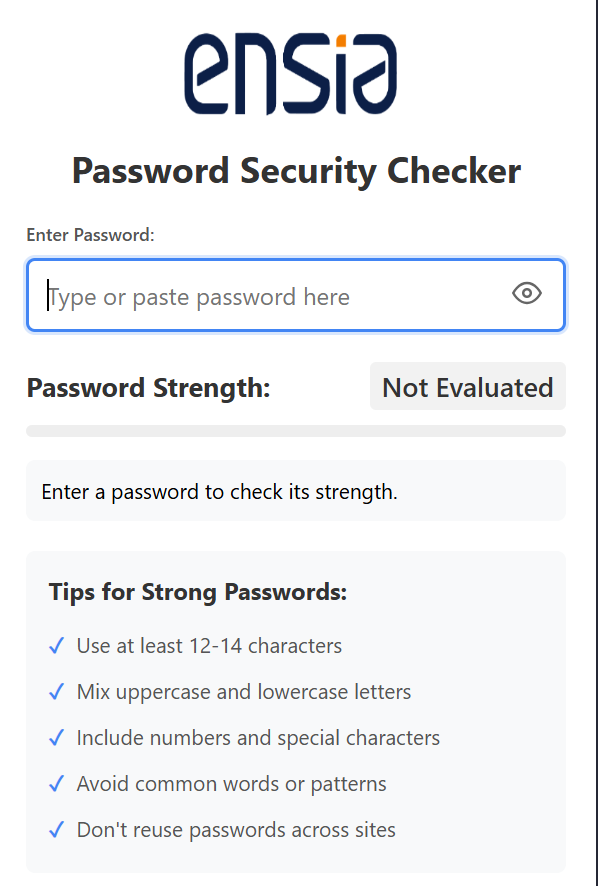
\includegraphics[width=0.45\textwidth]{type.png}
    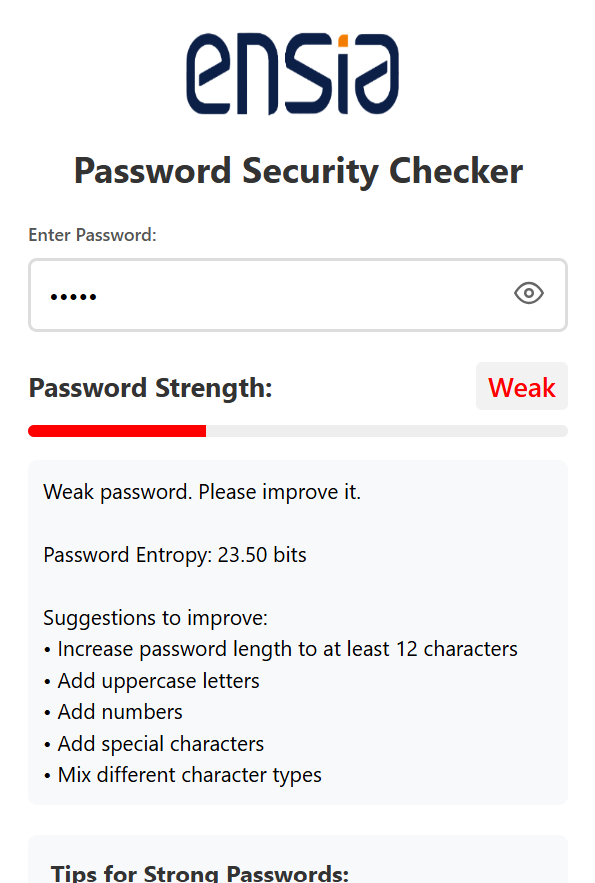
\includegraphics[width=0.45\textwidth]{low.png} \\
    \hline
    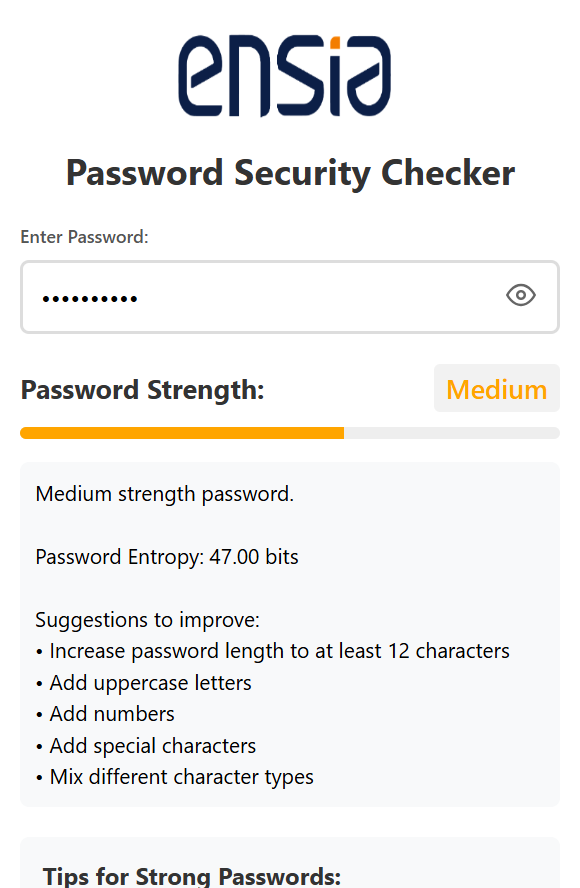
\includegraphics[width=0.45\textwidth]{medium.png}
    \hline
    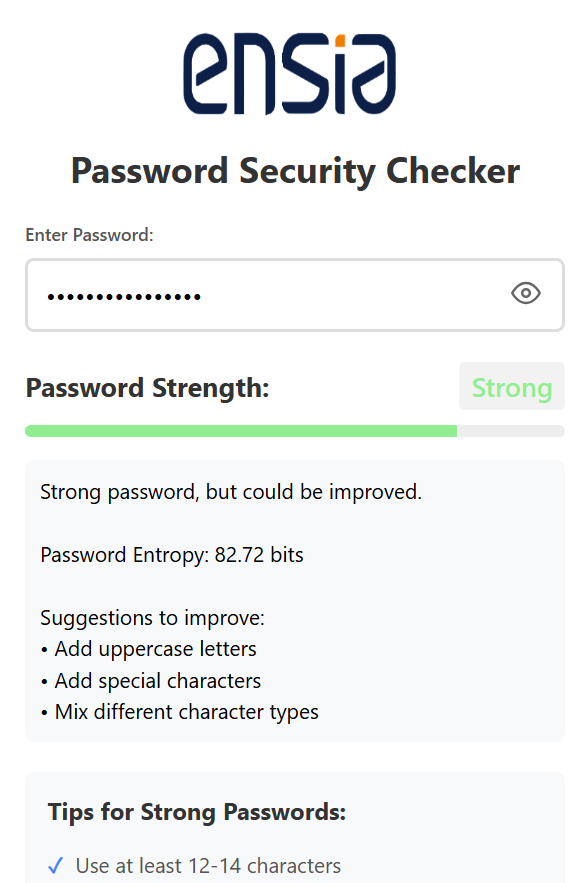
\includegraphics[width=0.45\textwidth]{strong.png} \\
    \hline
  \end{tabular}
  \caption{\extensionname\ Interface and Feature Demonstrations}
\end{table}
\begin{table}[H]
  \centering
  \begin{tabular}{|c|c|}
    \hline
     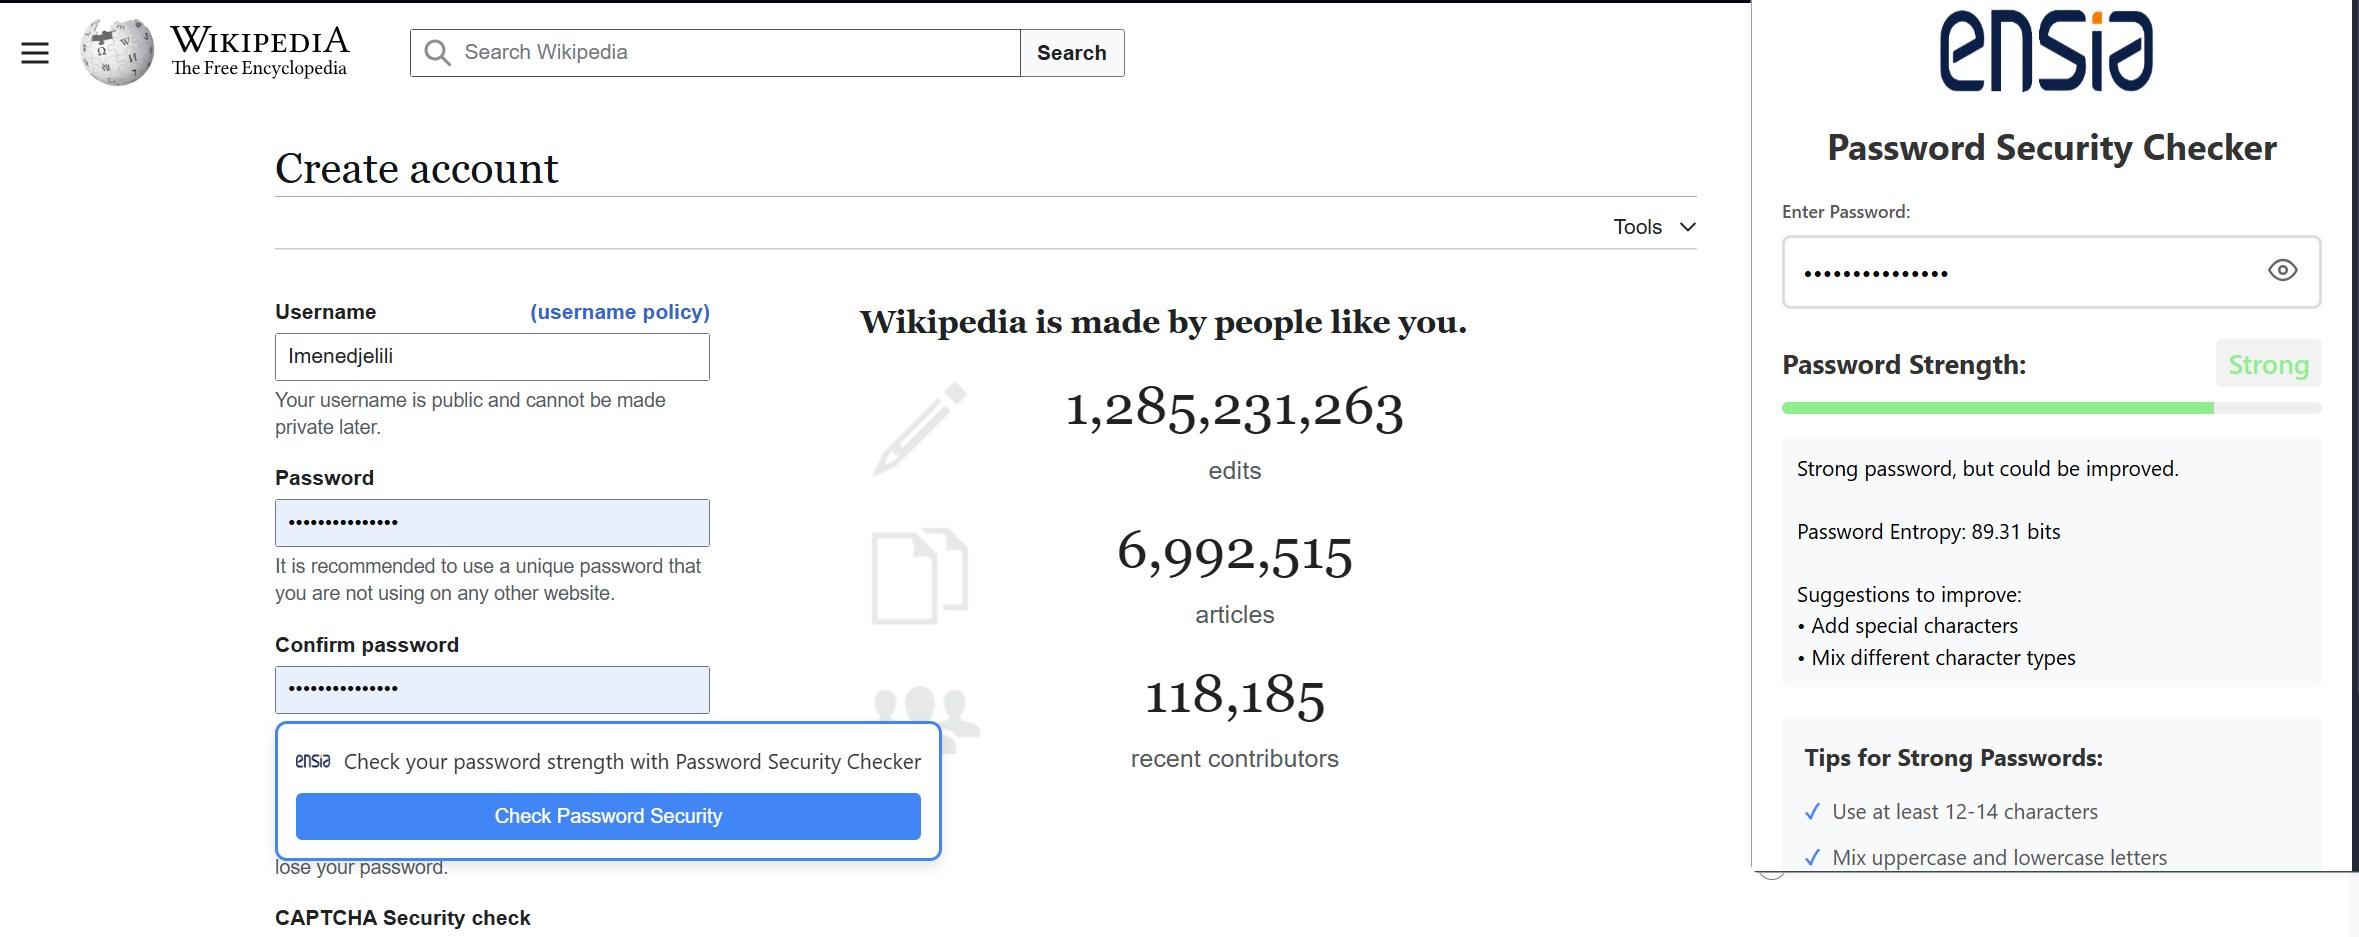
\includegraphics[width=0.45\textwidth]{checker.png} &
    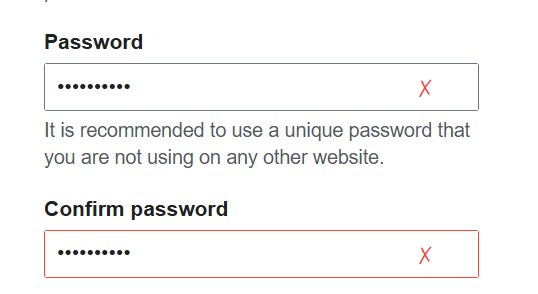
\includegraphics[width=0.45\textwidth]{red.png} \\
    \hline
  \end{tabular}
  \caption{\extensionname\ Interface and Feature Demonstrations}
\end{table}

\chapter{Links}
Key links related to the project:

\begin{itemize}
    \item \textbf{GitHub Repository:} Access the source code and project history. \newline
    \url{https://github.com/imenedjelili/CNS-Project---Secondary}
    \item \textbf{Demo Video:} A visual demonstration of the extension in use. \newline
    \url{https://drive.google.com/drive/folders/1MTh8wgICNQBM3qrUc3JF0slHRFNU7VEn?usp=sharing}
\end{itemize}


\end{document}